%!TeX TS-program = Lualatex
%!TeX encoding = UTF-8 Unicode
%!TeX spellcheck = en
%!BIB TS-program = biber
% -*- coding: UTF-8; -*-
% vim: set fenc=utf-8
%%%%%%%%%%%%%%%%%%%%%%%%%%%%%%%%%%%%%%%%%%%%%%%%%%%%%%%%%%%%%%%%%%%%%
\documentclass[11pt]{article}
\usepackage[utf8]{inputenc}
\usepackage{times}
\usepackage{wrapfig}
\usepackage{graphicx}
\usepackage{floatrow}
\usepackage{multicol}
\usepackage{amsmath}


\oddsidemargin -0.5in		% margin, in addition to 1" standard
\textwidth 7.5in		% 8.5" - 2*(1+\oddsidemargin)

\topmargin -1in		% in addition to 1.5" standard margin
\textheight 9.75in 		% 11 - ( 1.5 + \topmargin + <bottom-margin> )

\columnsep 0.25in

\parindent 0pt
\parskip 12pt

\flushbottom \sloppy
\pagestyle{empty} % No page numbers
%%%%%%%%%%%%%%%%%%%%%%%%%%%%%%%%%%%%%%%%%%%%%%%%%%%%%%%%%%%%%%%%%%%%%
\usepackage[
%style=chem-acs,
style=numeric,						% numeric style for reference list
citestyle=numeric-comp,
%style=alphabetic-verb,
giveninits=false,
maxbibnames=1,
%firstinits=true,
%style=apa,
%maxcitenames=1,
%maxnames=3,
%minnames=1,
%maxbibnames=99,
dateabbrev=true,
giveninits=true,
%uniquename=init,
url=false,
doi=false,
isbn=false,
eprint=false,
texencoding=utf8,
bibencoding=utf8,
autocite=superscript,
backend=biber,
%sorting=none,
sorting=none,
sortcites=false,
%articletitle=false
]{biblatex}%

\bibliography{ref.bib}
%%%%%%%%%%%%%%%%%%%%%%%%%%%%%%%%%%%%%%%%%%%%%%%%%%%%%%%%%%%%%%%%%%%%%%
\newcommand{\mycaption}[1]{\caption*{#1}}

\usepackage{titlesec}
% \titlespacing*{<command>}{<left>}{<before-sep>}{<after-sep>}
\titlespacing*{\section}
{0pt}{1.5ex}{0.8ex}
\titlespacing*{\subsection}
{0pt}{0.9ex}{0.4ex}
\titlespacing*{\subsubsection}
{0pt}{0.5ex}{0.3ex}
\titlespacing*{\paragraph}{%
  0pt}{%              left margin
  0.0\baselineskip}{% space before (vertical)
  1em}%               space after (horizontal)

\usepackage{setspace}

\begin{document}

%%%-----------------------------------------------------------------
{\Large\bf 
Automatic detection of spiking motifs in multi-unit raster plots
}

%{\bf
%Anonymous submission for double-blind review. \\
%}
\hrule
%%SUMMARY
%%%-----------------------------------------------------------------
\textbf{Summary} %}
There has been a recent surge of interest for the detection of reoccurring spike patterns in multi-unit raster plots [Russo 2017, Stella 2019]. In this study, we introduce an extension of such detection models by introducing a generative model for the synthesis of raster plots. We deduce from this model an optimal detection method. This takes the form of a logistic regression coupled to a temporal convolution. We evaluate the capacity of this model to detect spiking motifs in synthetic data. This demonstrates in particular the high capacity of such code in separating spiking motif. finally, as this model is differentiable, we derive an automatic unsupervised learning method, as a gradient descent on lake loss function of a model that word decode and re-encode the roster plot using spike motifs. Such unsupervised learning is able to retrieve the synthetically generated spike motifs and we envision to use these on neurobiological data.
\vspace{.5cm}
\hrule
%---------------------------
\textbf{Additional Details.}%
%

%\vspace{-25pt}
%---------------------------
\begin{figure}[h!]%wrapfigure}{}{\textwidth}
%\subfloat[Multi-unit raster plot]{
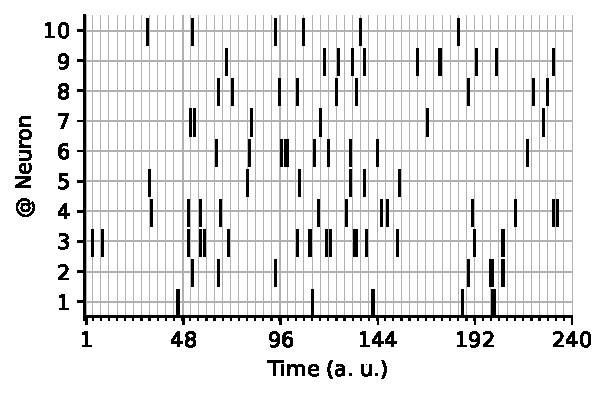
\includegraphics[width=.245\linewidth]{figure_1a_k.pdf}
%£}%
\hfill
%\subfloat[Raster plot of PGs]{
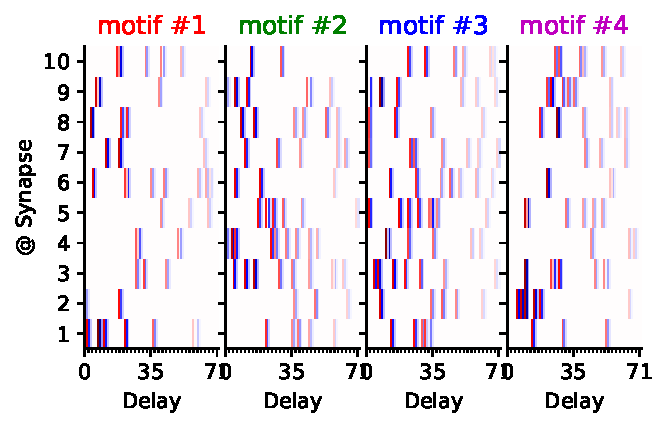
\includegraphics[width=.245\linewidth]{figure_1b.pdf}
%}%
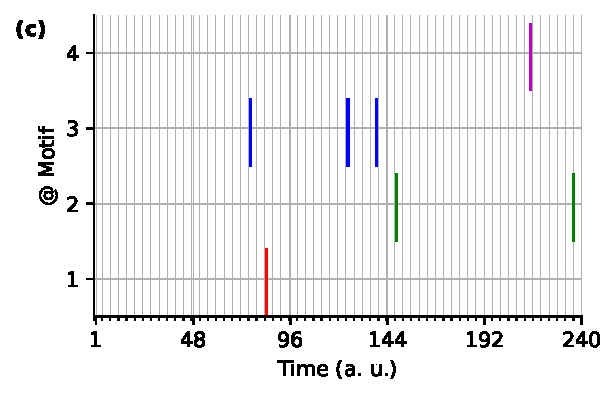
\includegraphics[width=.245\linewidth]{figure_1c.pdf}
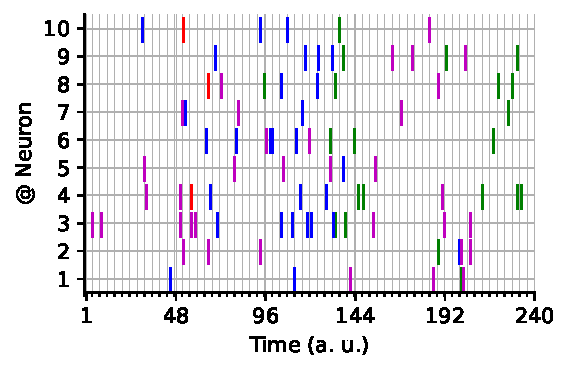
\includegraphics[width=.245\linewidth]{figure_1a.pdf}
%\vspace{-55pt}
{
\caption{A multi-unit raster plot is generated as the superposition of repeated spiking motifs. For illustration, we show here a superposition of $4$ different motifs, each denoted by a different color, and on a synaptic space of $10$ neurons. This superposition is then used to draw a raster plot on the the multi-unit address space. This defines a generative model for the synthesis of raster plots which, in turn, can be inverted to define an inference model for their efficient detection.
}
\label{fig:1}
}
\vspace{-5pt}
\end{figure}%wrapfigure}
%---------------------------
%
% * Limit : not online - in the future it is a model of a neuron
%
In general, a spiking neuron is defined on the one hand by the equations governing the evolution of its membrane potential dynamics on its soma and on the other hand by the characterization of the synaptic contacts on its dendritic tree. A classical characterization consists in detailing the synaptic weights of each synaptic contact on the dendritic tree. A more detailed examination of these synaptic contacts reveals the added importance of hetero-synaptic delays, i.e., the precise timing from synaptic activation to its integration into the soma, and how this changes the network's dynamics~\citep{Izhikevich06}. Thus, we can parameterize each neuron by the set of tuples defining the weight and delay of each synaptic contact. By discretization of time (with here an arbitrary unitary time unit), we can also define the dendrite as a matrix giving the weight corresponding to the different delays $d \in [0, D]$ (where $D$ is the maximum delay) on different pre-synaptic addresses $a \in [1, N]$ defining the list of the $N$ dendrites. We will denote as $W(a, d)$ these weights. When a neuron is activated by a discharge pattern that corresponds to this specific set of delays and addresses, the discharge probability will increase. Following the observations of~\citet{Izhikevich06}, let us assume that such precise discharge pattern defines a polychronous group (PG). Assuming that we know there exists $M$ such groups, we will define as $b \in [1, M]$ the address of a PG and as $W_b$ the corresponding weight matrices. This allows then to derive a generative model for raster plots (see Figure~\ref{fig:1}).

Indeed, the probability of firing of a neuron $a$ at a given time $t$ can be understood as a Bernoulli trial whose (only) parameter is a bias $p(t, a) \in [0, 1]$. Assuming that the presence of PGs is conditionally independent, this bias can be written as the combination of these factors, whose values are given by the corresponding weights. PGs may be activated independently at random times and  we write that $B(b, t)=1$ if $b$ is activated at $t$ (and else $B(b, t)=0$). We can thus write the probability bias as %the joint probability given these factors as 
$%$
p(t, a) = \sigma\big(W_0 + \sum_{b, t} B(b, t) \cdot W_b(a, t-d) \big)  
$, %$
where $\sigma$ is the sigmoid function. We will further assume that the weights are balanced (their mean is zero) and that $W_0$ is a bias such that $p_0=\sigma(W_0)$ is the average background firing rate. Conveniently, one can write this summation as a one-dimensional temporal convolution operator such that we may simply write $p = \sigma(W_0 + B \ast W )$ where  $p\in [ 0, 1]^{N\times T}$ and $B\in \{0, 1\}^{M\times T}$ is the raster plot corresponding to the temporal activation of the PGs. Finally, we obtain the raster plot $A\in \{0, 1\}^{N\times T}$ by drawing spikes using independent Bernoulli trials $A \sim \mathcal{B}(p)$. Note that, depending on the shape of the kernels, the generative model can model a Poisson process, generate rhythmic activity or more generally propagating waves. This formulation thus defines a simple generative model for raster plots as a combination of independent PGs. 

%---------------------------
\begin{wrapfigure}{r}{.275\textwidth}
\vspace{-15pt}
% ❯ git add figure_N_PG_time.pdf figure_N_PGs.pdf figure_N_pre.pdf
%\subfloat[]{
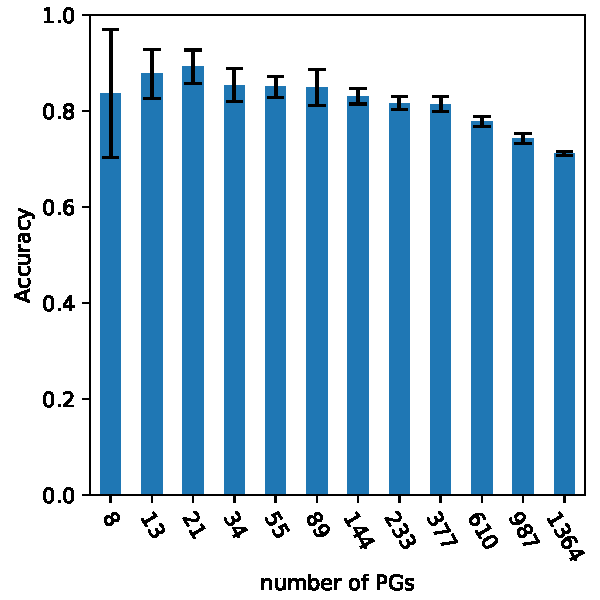
\includegraphics[width=\linewidth]{figure_N_PGs.pdf}
%}%
%\subfloat[]{\includegraphics[width=.49\linewidth]{Figures/fig_methods_nat.pdf}}%
\vspace{-25pt}
{
\caption{Accuracy of PG detection as a function of the number $M$ of kernels.
}
\label{fig:2}
}
\vspace{-10pt}
\end{wrapfigure}
%---------------------------
This generative model allows to define an inference model for guessing sources $B$ when observing a raster plot $A$. This assumes that we know the PGs as defined by the $W_b$ matrices. The underlying metric is the binary cross-entropy, as used in the logistic regression model. In particular, if we consider PG kernels with similar decreasing exponential time profile, we can prove that this is similar to %finding the tuning function of L-NL neurons, as used in 
the method of~\citet{berens_fast_2012}. In our specific case, the difference is that the regression is performed in both dendritic and delay space by extending the summation using a temporal convolution operator. Using this forward model, it possible to estimate the logit (inverse of a sigmoid) $\hat{B}(b, t)$ for the presence of a PG of address $b$ and at time $t$ by using the transpose convolution operator. It thus comes that when observing $A$, then one may infer $\hat{B} = A \ast W^T$ and select the most activated items. To quantify the efficiency of this operation, we generated $M=55$ synthetic PGs as random independent kernels over $128$ presynaptic inputs and $D=127$ possible delays. We drew random independent instances of $B$ with a length of $T=1000$ time steps and with on average $2.0$ occurrences each. This allowed us to generate raster plots which we use to infer $\hat{B}$. We compute the accuracy as the rate of true positive detections and observe on average $\approx 98\%$ correct PGs both for the address and %(exact) 
timing.

%---------------------------
\begin{wrapfigure}{r}{.275\textwidth}
\vspace{-10pt}
% ❯ git add figure_N_PG_time.pdf figure_N_PGs.pdf figure_N_pre.pdf
%\subfloat[]{
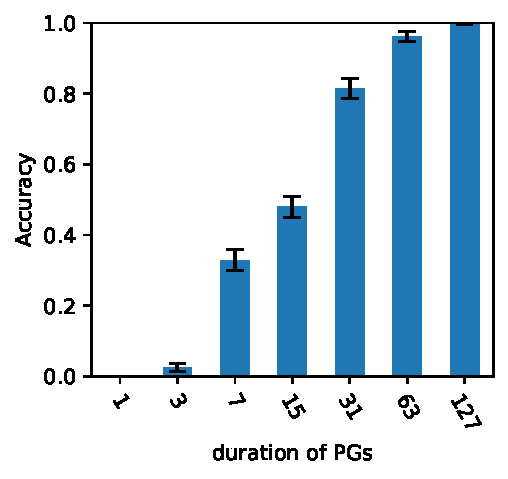
\includegraphics[width=\linewidth]{figure_N_PG_time.pdf}
%}%
%\subfloat[]{\includegraphics[width=.49\linewidth]{Figures/fig_methods_nat.pdf}}%
\vspace{-25pt}
{
\caption{Accuracy of PG detection as a function of the temporal depth $D$ of kernels.
}
\label{fig:3}
}
\vspace{-15pt}
\end{wrapfigure}
%---------------------------
We further extended this result by showing how the accuracy would evolve as a function of the number of simultaneous PGs, while keeping the same frequency of occurrence. We show in Figure~\ref{fig:2} that the accuracy of finding the right PG is still above $80\%$ accuracy with more than $1364$ PGs. Moreover, we show in Figure~\ref{fig:3} that (with $M=55$ PGs fixed) the accuracy increases notably as the temporal depth $D$ of the PG kernel increased, demonstrating quantitatively the potential of hetero-synaptic delays. These results were obtained while assuming that we know $W$. However, this is in general not the case, for instance when observing the raster plot of a population of neurons. Inspired by the k-means algorithm, it is possible to devise a self-supervised learning algorithm. Our preliminary results show that it is possible to retrieve PGs embedded in the data, yet that further analysis is necessary to improve the convergence of the algorithm. In particular, it seems promising to use a sparseness constraint in the inference mechanism such as to remove spurious correlations in the inference.


% \section{Theoretical framework for polychronous group detection}


%\vspace{-55pt}
%\subsubsection*{References}
\textbf{References.} %}
%{
%\small
%\footnotesize
%\begingroup
%\setstretch{0.75}
%\setlength\bibitemsep{1pt}
%\begingroup
%\setstretch{0.75}
%\setlength\bibitemsep{1pt}
%\printbibliography[heading=none]
%\printbibliography
%\endgroup
%\endgroup
%}
\cite{Izhikevich06}~\href{http://izhikevich.org/publications/spnet.htm}{Izhikevich, \emph{Neural Computation}, 2006.}
\cite{berens_fast_2012}~\href{https://www.jneurosci.org/content/32/31/10618}{Berens et al., \emph{Journal of Neuroscience}, 2012.}
\end{document}



%
\printbibliography
\end{document}
